\documentclass[../main.tex]{subfiles}
\begin{document}

\subsection*{Exercise 1 – Understanding tire data}
\textbf{Q. Plot the raw data in different graphs, specifically focusing on $\kappa$, $\alpha$, $\gamma$, $\fz$\ and pressure $P$. Comment on what you see. What is, according to you, the main target of these tests?}

        \begin{figure}[ht]
        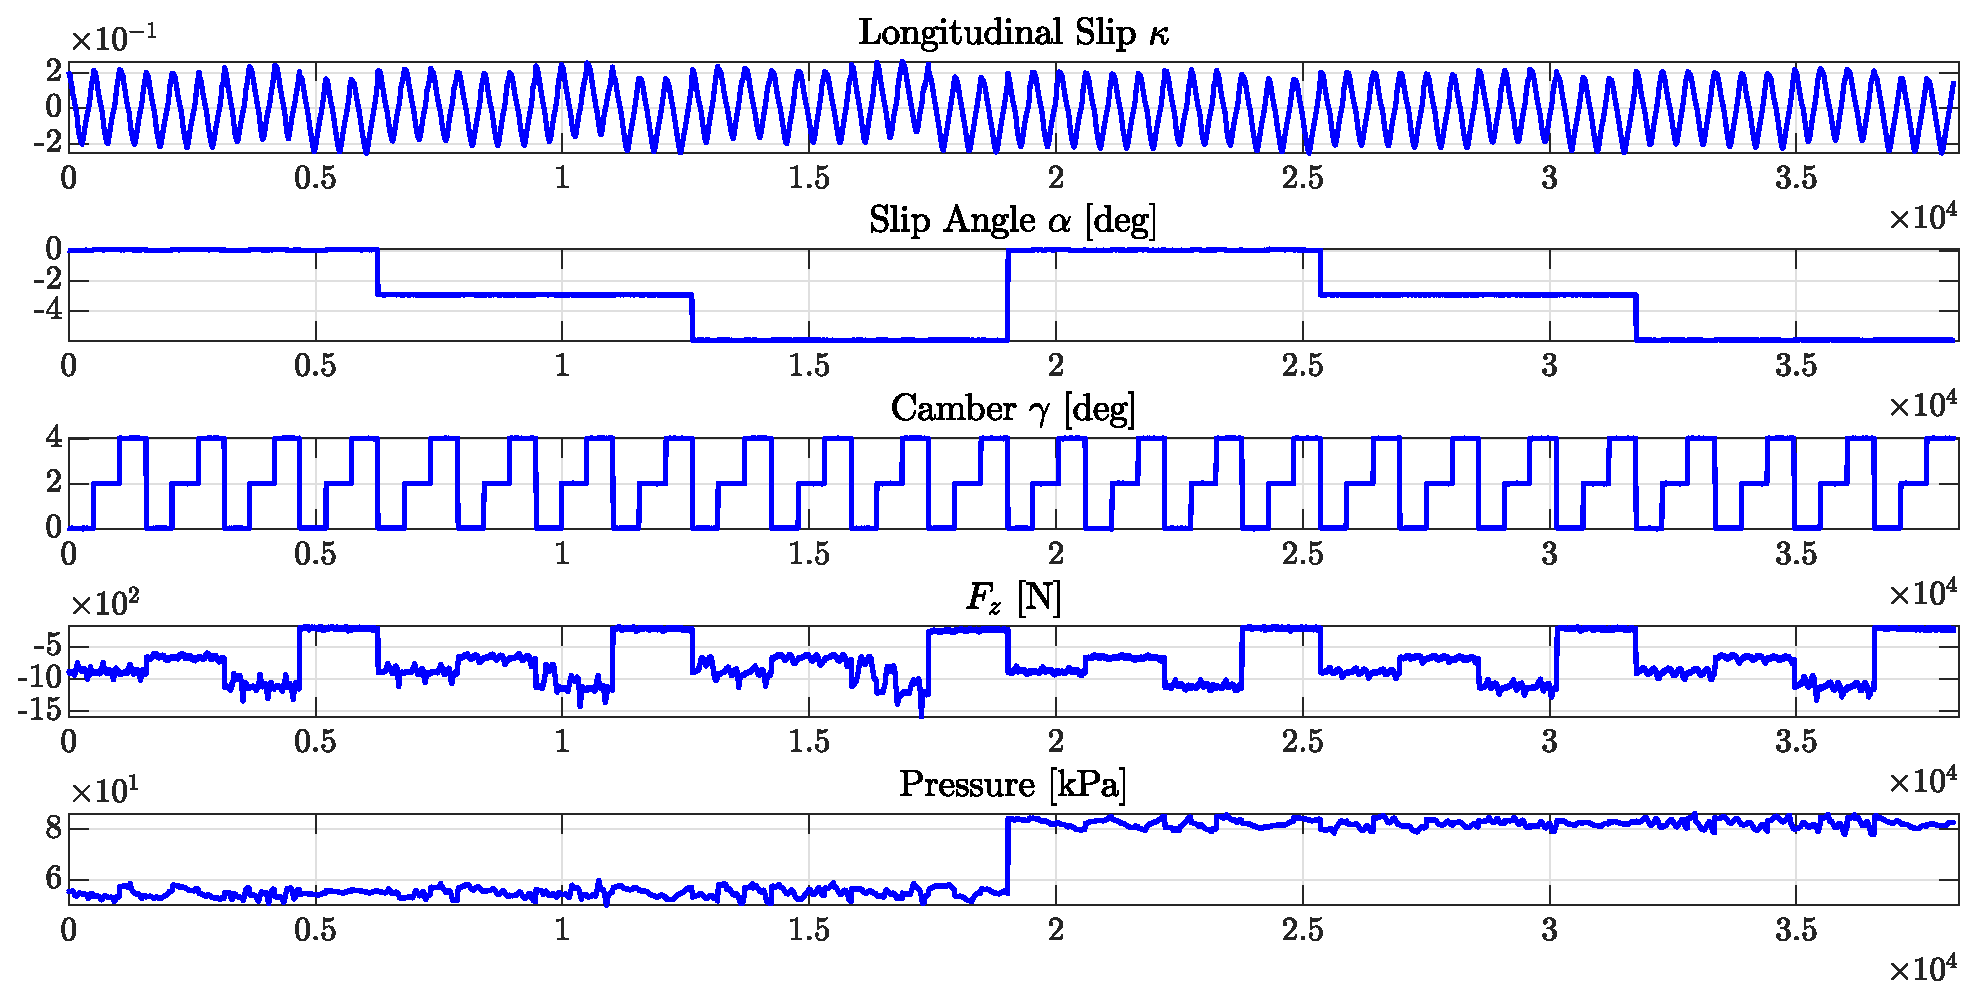
\includegraphics[scale=0.4]{ex2/ex-21.eps}
        \centering
        \caption{raw data}
        \label{rd}
        \end{figure}

From the five plotted variables if Figure \ref{rd}, it appears that the slip angle, camber, vertical force, and pressure are all showing repeat patterns. That means that those four variables are controlled to measure and test the longitudinal slip $\kappa$.

\textbf{Q. Focus on the data with $\alpha$ =0 and $\gamma$ =0, and plot the curves $\fx$\ vs $\kappa$ for each of the 4 vertical loads $\fz$\ used in the experiments. Plot the 4 curves on the same graph, with different colors. Comment on what you see.}

        \begin{figure}[ht]
        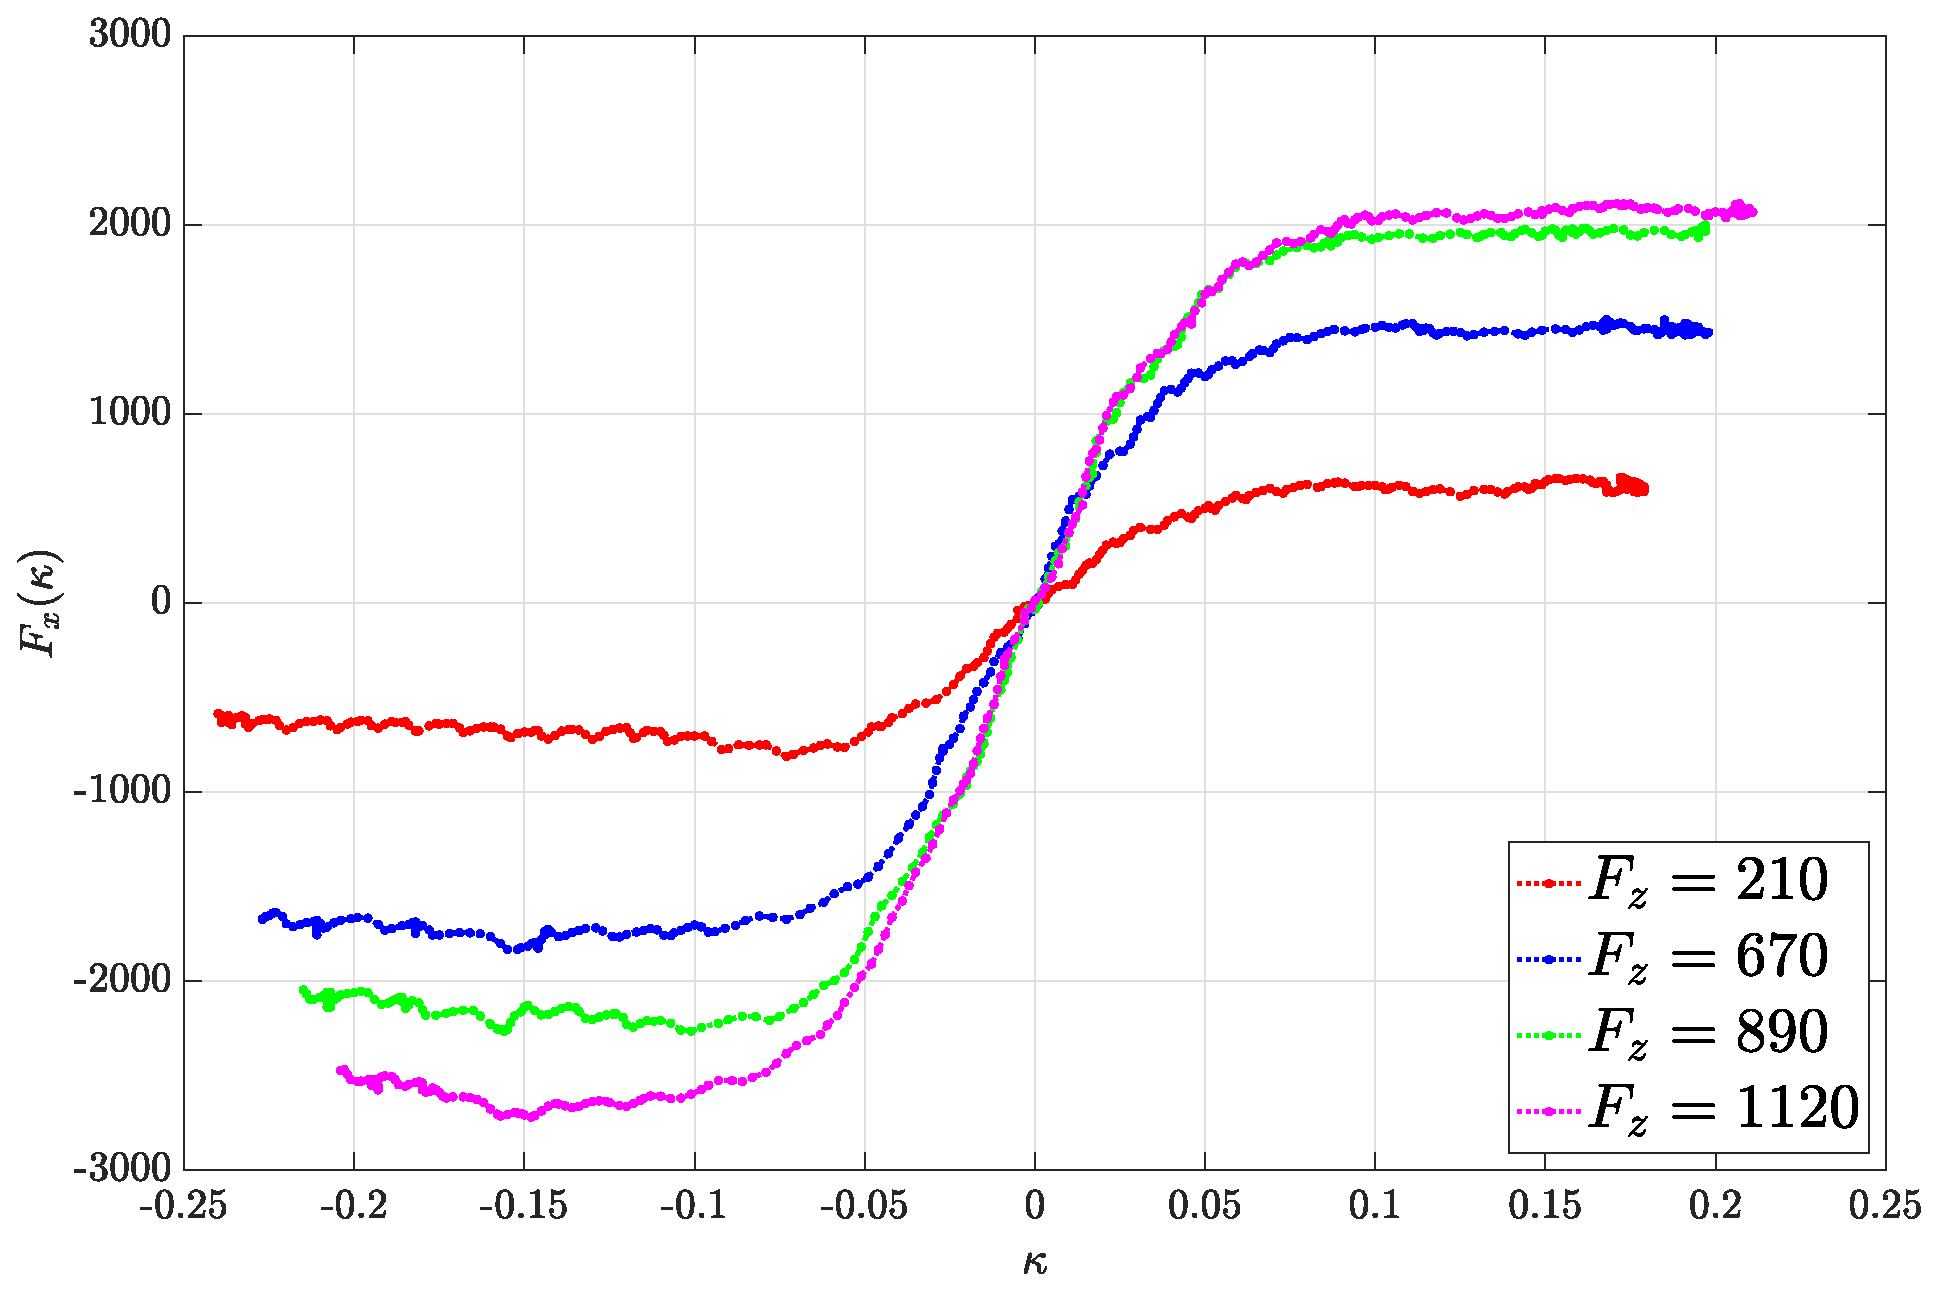
\includegraphics[scale=0.35]{ex2/ex-22.eps}
        \centering
        \caption{$\kappa$ vs $\fx$\ based on vertical force}
        \label{lsvlf}
        \end{figure}

Figure \ref{lsvlf} suggests that the Longitudinal Force $\fx$\ increases with the vertical force $\fz$. There is some dependency on the vertical force. If you double the vertical force, it does not mean the longitudinal force will double. In some parts there is a linear dependency, but in others it is not the case.

\textbf{Q. Focus on the data with $\gamma$ =0 and $\fz$\ = 150 lbf $\approx$ 670N, and plot the curves $\fx$\ vs $\kappa$ for each of the 3 side slip angles $\alpha$ used in the experiments. Plot the 3 curves on the same graph, with different colors. Comment on what you see.}

The Longitudinal Force $\fx$\ in Figure \ref{lsvlfv} shows an inverse relationship with the side slip angle. 
        \begin{figure}[ht]
        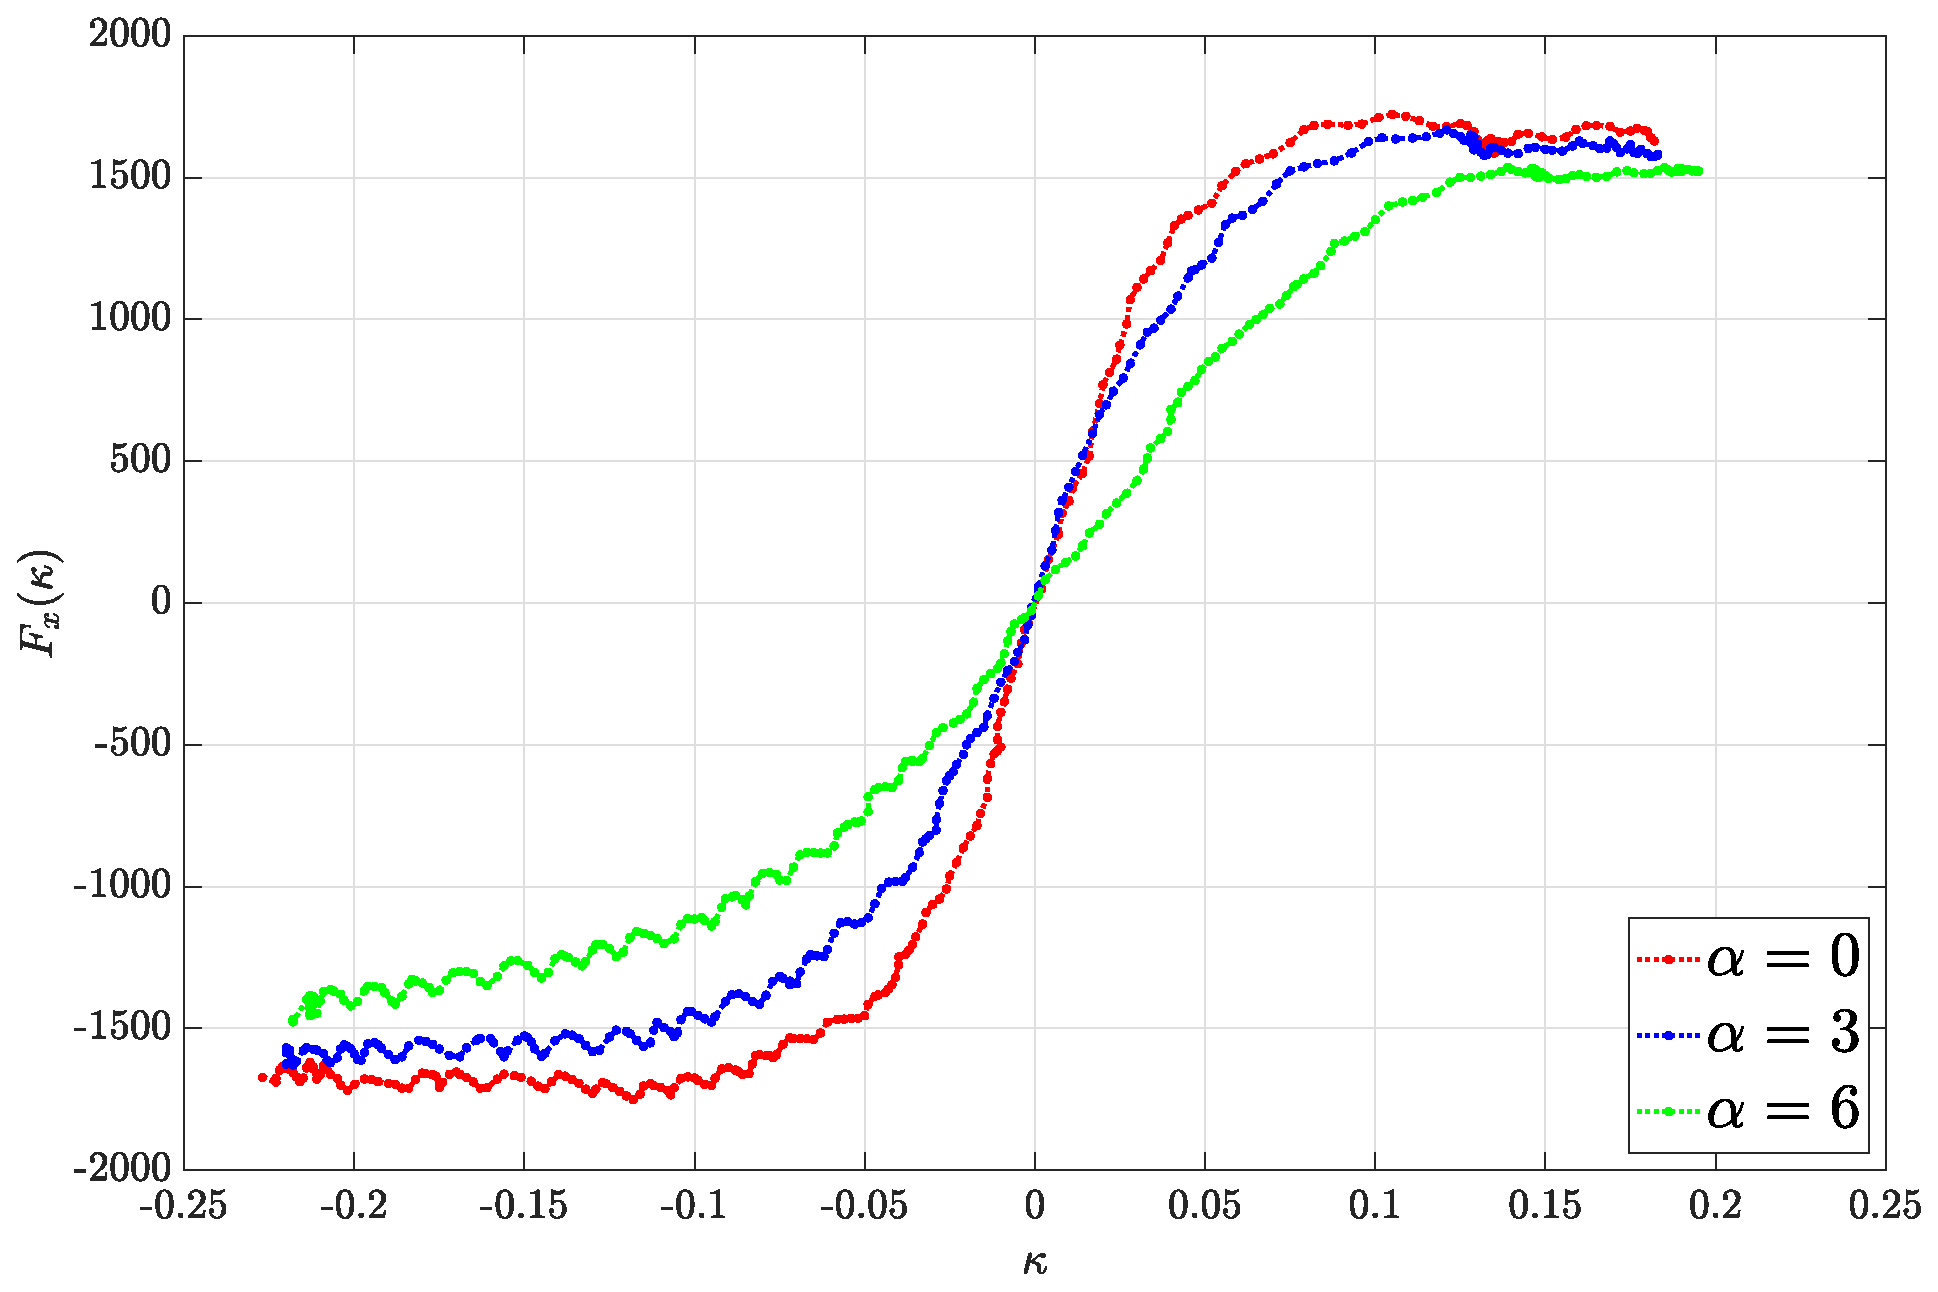
\includegraphics[scale=0.35]{ex2/ex-23.eps}
        \centering
        \caption{$\kappa$ vs $\fx$\ at vertical force = 670 based on slip angle}
        \label{lsvlfv}
        \end{figure}

\subsection*{Exercise 2 - Fitting tire data}

\textbf{Q. First consider the data with $\fz$\ = $\fzz$\ =890N, $\gamma$ =0 and $\alpha$ =0, and fit the coefficients X1 = \{$\pcxo$, $\pdxo$, $\pexo$ , $\pexf$, $\pkxo$, $\phxo$, $\pvxo$\}. Build a function $resid pure \fx$ that calculates the pure longitudinal force $\fxz$\ and the residuals. Plot the fitted curve $\fx$\ vs $\kappa$ that you obtained in these nominal conditions, together with the raw data.}

        \begin{figure}[ht]
        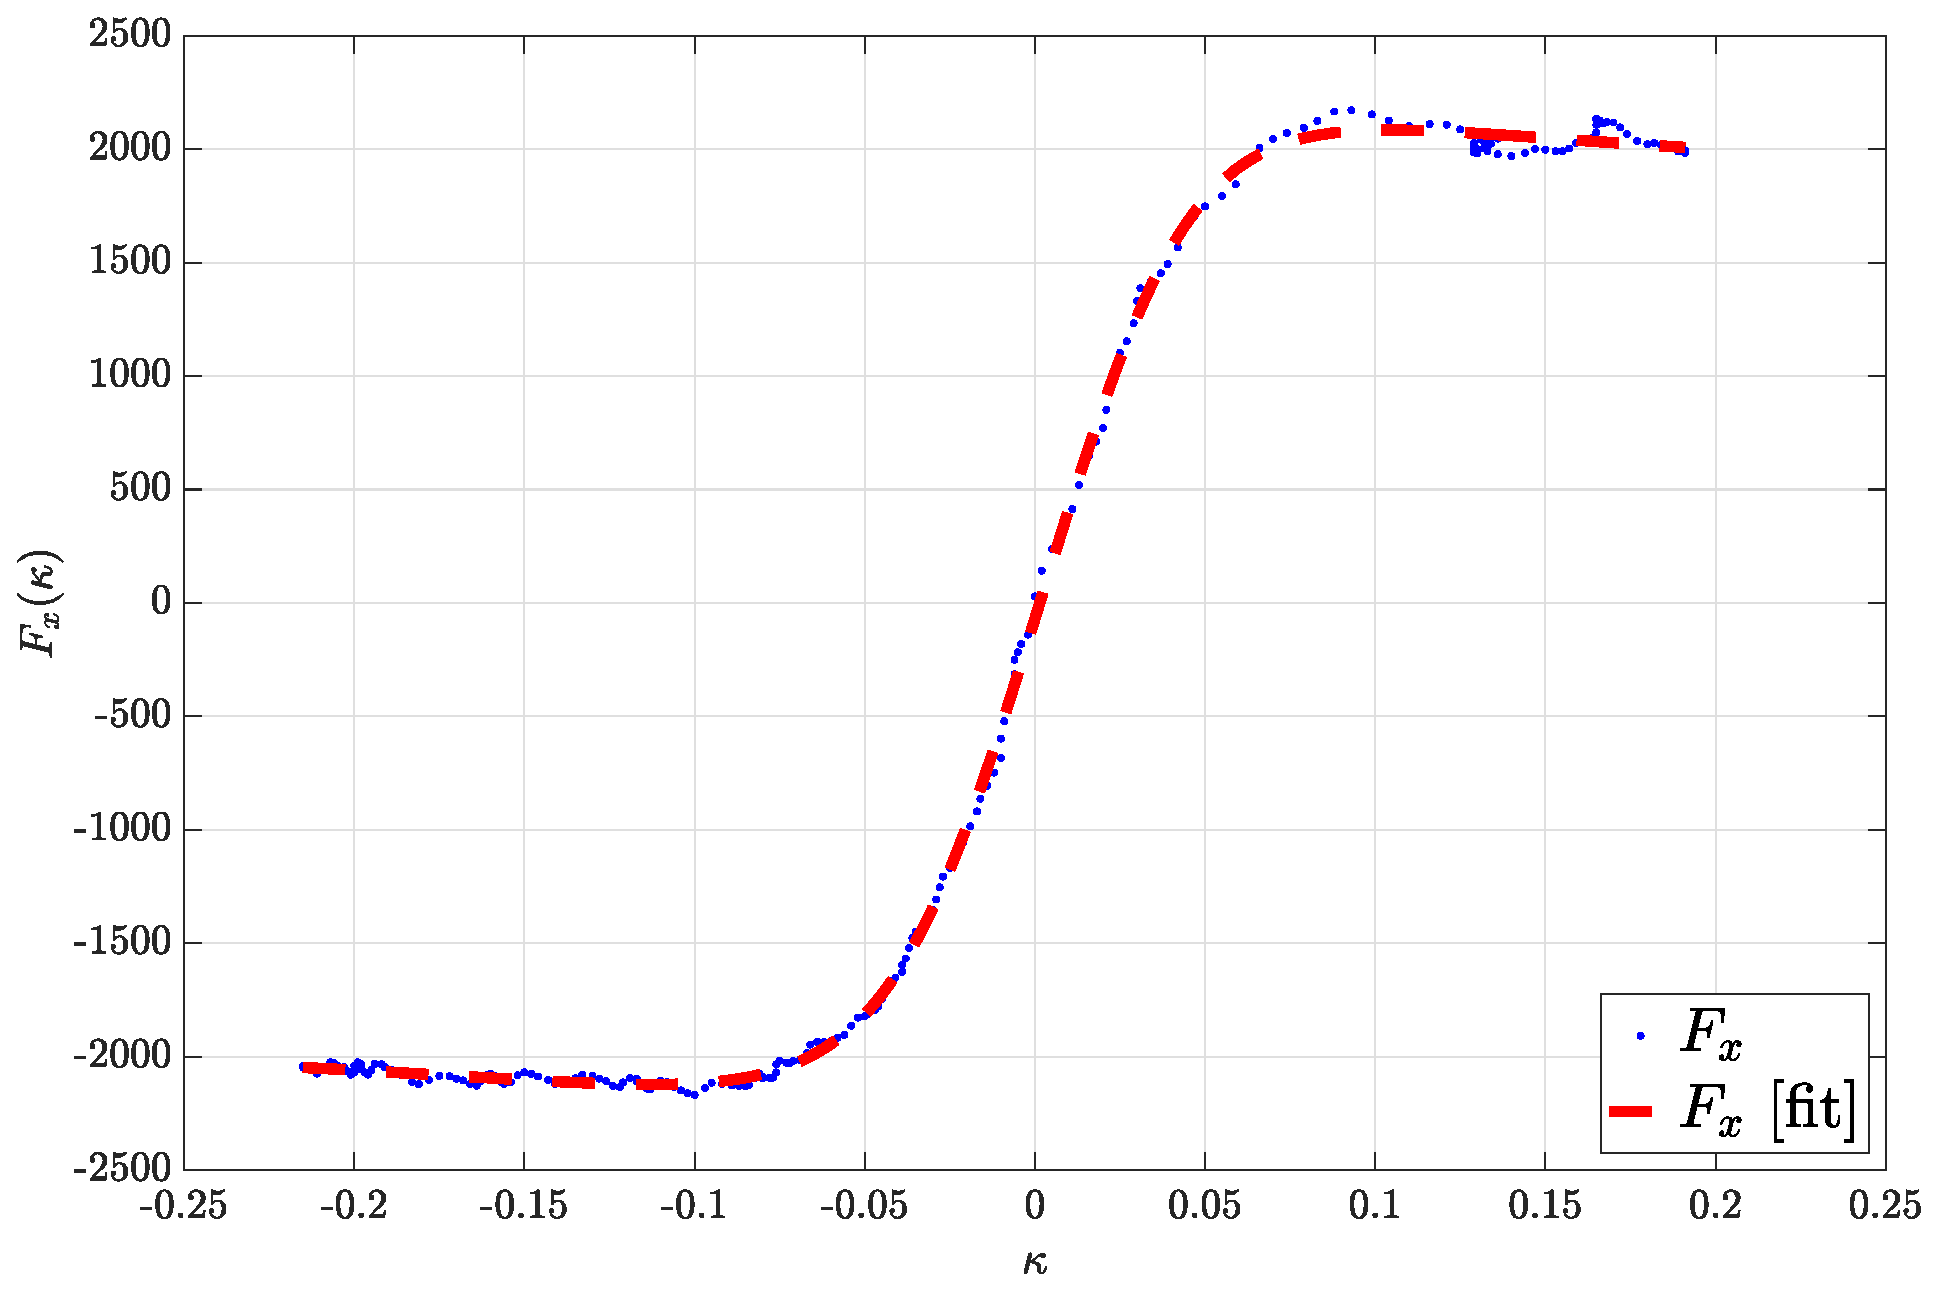
\includegraphics[scale=0.35]{ex2/ex-24.eps}
        \centering
        \caption{Fitted $\fxz$\ after optimizing first 7 parameters compared to test data vs $\kappa$}
        \label{faopt}
        \end{figure}

In Figure \ref{faopt}, the data was filtered based on the following criteria: $\fzz$\ = 890, $\alpha$\ = 0, $\gamma$\ = 0 and $P$ = 82kPa. The first 7 coefficients were optimized using the $fmincon$ function in Matlab. The 7 coefficients initial guess vector was chosen randomly. The initial guess vector has proven to be quite important as running the code multiple times showed a curve that did not fit the data at all, which means the optimizer was stuck at a local minima. However, most of the time the initial guess gave a very good fit that converged to the correct global minima. 


\textbf{Q. Now consider the data with the 4 different values of $\fz$, but still $\gamma$ = 0 (and $\alpha$ = 0). This enables the fitting of the parameters: X2 =\{$\pdxt$,$\pext$,$\pextt$,$\phxt$,$\pkxt$,$\pkxtt$,$\pvxt$\}. You can build another function so as to use the optimal parameters X1,opt found before for the coefficients already computed. Plot the fitted and raw curves $\fxz$\ vs $\kappa$ for the 4 values of $\fz$\ and comment the results.}

\end{document}